\subsection{Modell der Seite}
    % TODO: UML Diagramm der Seite, dann ist es auch ein Modell
    Abbildung \ref{image:findingTeachersModelOverview} zeigt einen
    Ausschnitt der Übersichtsseite des Studienportal "``B.A. Bildungswissenschaft"',
    anhand dessen das Modell der Seite beschrieben wird.
    Eine schematische Darstellung ist außerdem in Abbildung
    \ref{image:findingTeachersModelUml} zu sehen.

    \begin{figure}[htb]
        \centering
        
\includegraphics[width=\textwidth]{../resources/findings/case-study-1/model/overview.png}
        \caption{Ausschnitt aus einer Seite: Lehrende und Betreuende}
        \label{image:findingTeachersModelOverview}
    \end{figure}

    Die Webseite lässt sich in verschiedene Bereiche aufteilen.
    Zunächst einen Kopfbereich, der auf der linken Seite das Logo
    der {\fernUni} und rechts einige Links zu den verschiedenen
    Bereichen dieser Site.
    Das Logo ist gleichzeitig ein Link zur Hauptseite der Universität.

    Direkt unter dem Kopfbereich befindet sich der Name des Studienportals,
    welcher gleichzeitig ein Link auf Hauptseite der Website darstellt.

    Darunter befindet sich auf der linken Seite ein weiterer Navigationsbereich,
    der Verweise auf die Unterseiten dieses Bereichs enthält.

    Rechts daneben findet sich zunächst der Titel der Seite,
    gefolgt von einem kurzen einleitenden Absatz.

    Darunter befindet sich die Liste aller Lehrenden und Betreuenden.
    Jeder Mitarbeiter ist durch eine Reihe an Informationen dargestellt.
    Neben einem Bild ist das der Name des Lehrgebiets, in dem er tätig ist.
    Dieser Name ist außerdem ein Link auf eine Seite über dieses Gebiet.
    Es folgen der Name des Mitarbeiters,
    sowie einige Kontaktinformationen.
    Dies können eine E-Mail-Adresse, eine Telefonnummer
    und bei einigen wenigen Kontakten auch eine Faxnummer und ein Raum sein.

    \begin{figure}[htb]
        \centering
        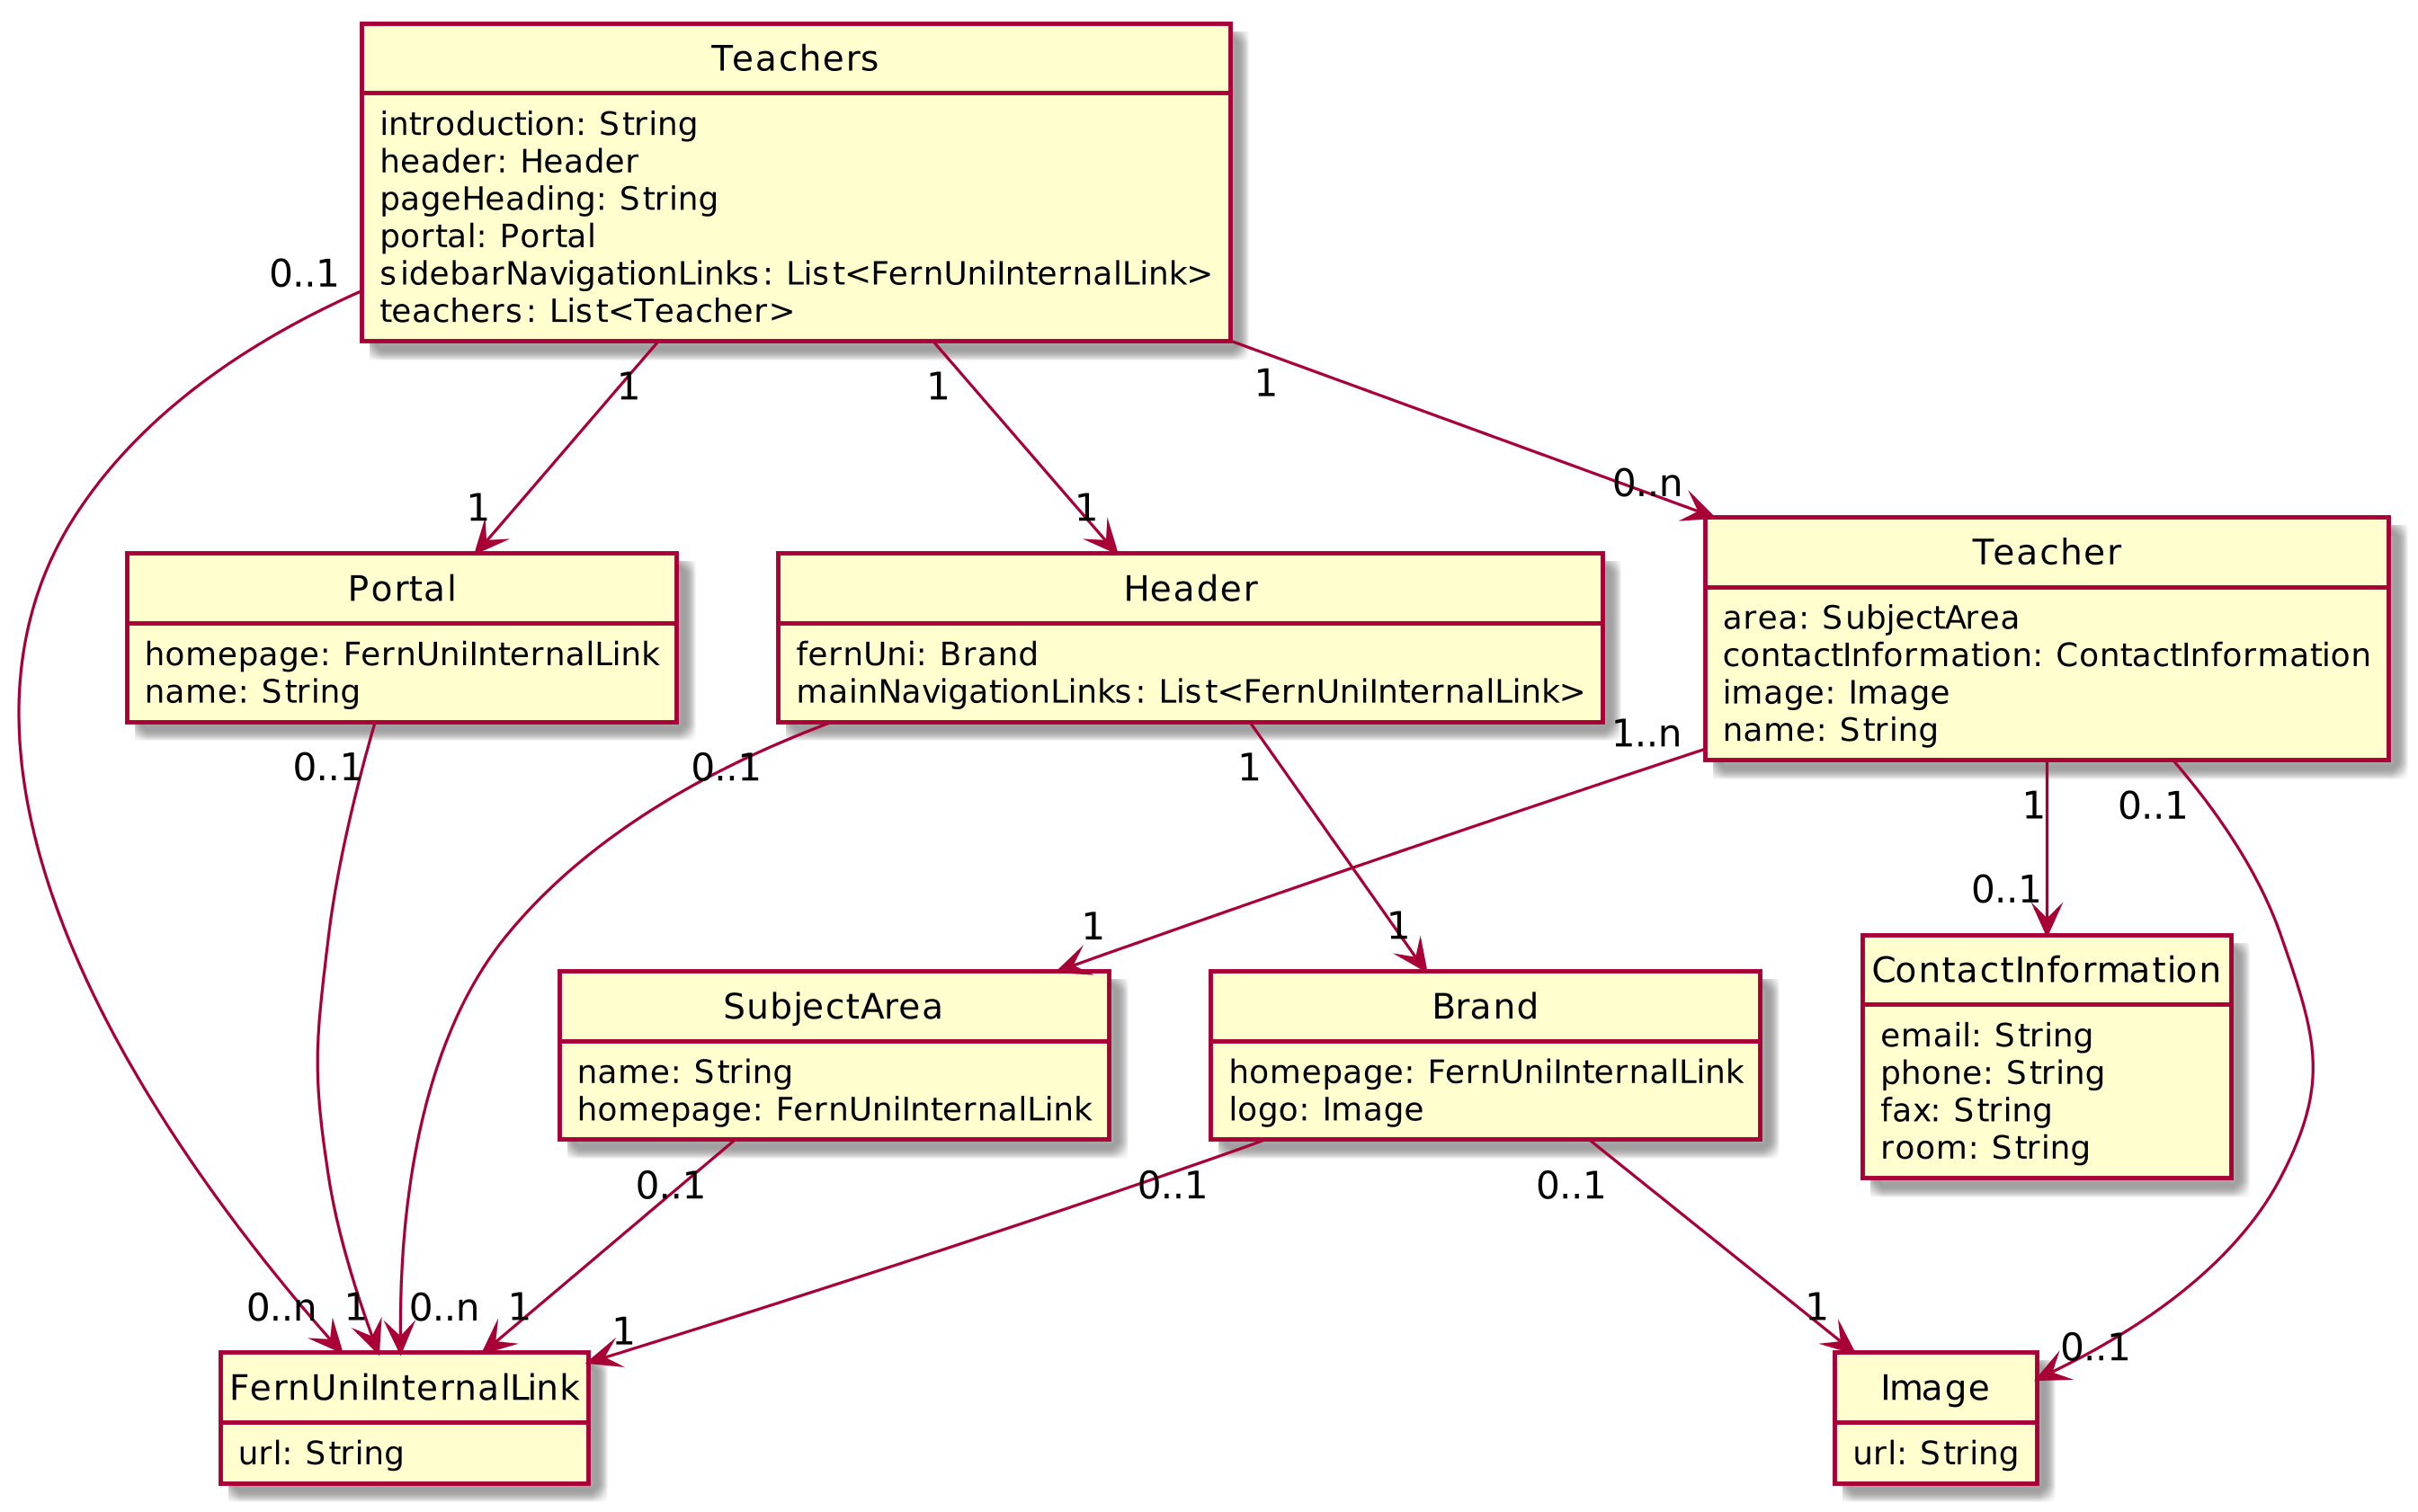
\includegraphics[scale=\imageScalingFactor]{../resources/findings/case-study-1/model/model.png}
        \caption{Schematische Darstellung der Seite Lehrende und Betreuende}
        \label{image:findingTeachersModelUml}
    \end{figure}